\documentclass{beamer}

\usepackage{amsmath, amssymb, graphicx, hyperref}
\usepackage[english]{babel}
\usepackage{xcolor}
\usepackage[T1]{fontenc}

\title{Importance Sampling}
\subtitle{English translation of the Polish original}
\author{Natalia Bednarz, Aleksandra Bieniek, Max Stróżyk}
\date{21 January 2025}

\begin{document}

\begin{frame}
    \titlepage
\end{frame}

\begin{frame}{Introduction to IS}
    \textbf{Importance Sampling (IS)} is a simulation technique used to estimate rare events.
    
    \vspace{0.5cm}
    \textbf{Objective:}
    \begin{itemize}
        \item Classical Monte Carlo (MC) needs a very large sample to estimate rare-event probabilities precisely.
        \item IS reduces the number of samples needed for the same accuracy.
    \end{itemize}
\end{frame}

\begin{frame}{How does Importance Sampling work?}
    The main idea of IS is:
    \begin{enumerate}
        \item Change the probability distribution of the random variable $X$ to a \textit{biasing distribution} $f^*(x)$.
        \item Weight samples from $f^*(x)$ using the weight function $W(x)$:
        \[
        W(x) = \frac{f(x)}{f^*(x)},
        \]
        where $f(x)$ is the original distribution.
    \end{enumerate}

    \vspace{0.5cm}
    \textbf{Estimation:}
    IS estimates the event probability $P(X \geq t)$ as:
    \[
    P(X \geq t) = \mathbb{E}^*\big[W(X) \cdot \mathbb{I}(X \geq t)\big],
    \]
    where $\mathbb{E}^*$ denotes expectation under $f^*(x)$.
\end{frame}

\begin{frame}
    \textbf{Advantages of IS:}
    \begin{itemize}
        \item Focuses simulations on \textit{important} regions where rare events occur.
        \item Reduces estimator variance compared with classical MC.
        \item Uses a \textbf{biasing distribution} that increases the frequency of rare events.
    \end{itemize}

    \vspace{0.5cm}
    \textbf{Example:}
    \begin{itemize}
        \item Classical MC: few samples satisfy $X \geq t$, leading to high variance.
        \item IS: with a suitable $f^*(x)$, most samples satisfy $X \geq t$.
    \end{itemize}
\end{frame}

\begin{frame}
    \textbf{General definition of IS:}
    \[
    \mathbb{E}[g(X)] = \int g(x)f(x)dx = \int g(x)W(x)f^*(x)dx = \mathbb{E}^*[g(X)W(X)],
    \]
    where:
    \begin{itemize}
        \item $g(X)$ is the function of the random variable whose expectation is estimated,
        \item $f(x)$ is the original probability distribution,
        \item $f^*(x)$ is the biasing distribution,
        \item $W(x) = \frac{f(x)}{f^*(x)}$ is the weight function.
    \end{itemize}

    \vspace{0.5cm}
    \textbf{Variance of the IS estimator:}
    \[
    \text{Var}^*[g(X)W(X)] = \mathbb{E}^*[g^2(X)W^2(X)] - \left(\mathbb{E}^*[g(X)W(X)]\right)^2.
    \]
\end{frame}






\begin{frame}{Distribution-changing techniques}
    \vspace{0.5cm}
    \textbf{Scaling} and \textbf{Translation} are two basic ways to change distributions:
    \begin{itemize}
        \item \textbf{Scaling:} Rescale the random variable to concentrate probability mass in the region of interest.
        \item \textbf{Translation:} Shift the distribution to increase the number of samples in the rare-event region.
    \end{itemize}
\end{frame}

\begin{frame}{Scaling}
    \textbf{Scaling} rescales a random variable $X$ by a factor $a > 1$:
    \[
    X^* = aX.
    \]

    \textbf{Biasing distribution:}
    \[
    f^*(x) = \frac{1}{a}f\left(\frac{x}{a}\right),
    \]
    where $f(x)$ is the original distribution of $X$.

    \vspace{0.5cm}
    \textbf{Weighting:} The weight function $W(x)$ is the density ratio:
    \[
    W(x) = \frac{f(x)}{f^*(x)} = \frac{af(x)}{f(\frac{x}{a})}
    \]
\end{frame}

\begin{frame}{Scaling example: Weibull distribution}
    Consider a random variable $X$ with a Weibull distribution:
    \[
    f(x) = \frac{b}{\lambda}\left(\frac{x}{\lambda}\right)^{b-1} e^{-(x/\lambda)^b}, \quad x \geq 0.
    \]

    \textbf{Biasing distribution after scaling:}
    \[
    f^*(x) = \frac{b}{a\lambda}\left(\frac{x}{a\lambda}\right)^{b-1} e^{-\left(\frac{x}{a\lambda}\right)^b}.
    \]

    \textbf{Weight function:}
    \[
    W(x) = a^be^{-(1-a^{-b})(\frac{x}{\lambda})^b}
    \]
\end{frame}

\begin{frame}{Translation}
    \textbf{Translation} shifts a random variable $X$ \\ by $c$:
    \[
    X^* = X + c, \quad c > 0.
    \]

    \textbf{Biasing distribution:}
    \[
    f^*(x) = f(x - c),
    \]
    where $f(x)$ is the original distribution of $X$.

    \vspace{0.5cm}
    \textbf{Weighting:} The weight function $W(x)$ is the density ratio:
    \[
    W(x) = \frac{f(x)}{f^*(x)} = \frac{f(x)}{f(x - c)}.
    \]
\end{frame}

\begin{frame}{Translation example: Gaussian distribution}
    Consider a random variable $X$ with a normal distribution $N(0, 1)$:
    \[
    f(x) = \frac{1}{\sqrt{2\pi}} e^{-\frac{x^2}{2}}.
    \]

    \textbf{Biasing distribution after translation:}
    \[
    f^*(x) = \frac{1}{\sqrt{2\pi}} e^{-\frac{(x - c)^2}{2}}, \quad c > 0.
    \]

    \textbf{Weight function:}
    \[
    W(x) = e^{-\frac{c(2x - c)}{2}}.
    \]
\end{frame}

\begin{frame}{Comparison of Scaling and Translation}
    \begin{itemize}
        \item \textbf{Scaling:}
        \begin{itemize}
            \item Effective for homogeneous variables, such as the Weibull distribution.
            \item May spread probability mass into unwanted regions.
        \end{itemize}
        \item \textbf{Translation:}
        \begin{itemize}
            \item More effective for symmetric distributions, such as the Gaussian.
            \item Avoids the \lq\lq dimensionality effect\rq\rq \space encountered in scaling.
        \end{itemize}
    \end{itemize}
\end{frame}

\begin{frame}{Exponential Twisting}
    \textbf{Exponential Twisting (ET)} is an importance-sampling technique based on:
    \begin{itemize}
        \item changing the distribution of $X$ by \lq\lq twisting\rq\rq \space its density,
        \item using a distribution with a modified moment-generating function.
    \end{itemize}

    \vspace{0.5cm}
    \textbf{Objective:}
    \begin{itemize}
        \item ET minimizes estimator variance by optimally \textit{redirecting probability mass} toward important-event regions.
        \item It is particularly effective for rare-event estimation, where classical approaches may fail.
    \end{itemize}
\end{frame}

\begin{frame}
    \textbf{Density twisting:} Generate a new density $f^*(x)$ by twisting the original density $f(x)$:
    \[
    f^*(x) = \frac{e^{sx} f(x)}{M(s)},
    \]
    where:
    \begin{itemize}
        \item $M(s) = \mathbb{E}[e^{sX}]$ is the moment-generating function,
        \item $s > 0$ is the \textit{twisting} parameter, optimized to minimize estimator variance.
    \end{itemize}

    \vspace{0.5cm}
    \textbf{Weighting:} The weight function $W(x)$ for a sample $x$ is:
    \[
    W(x) = \frac{f(x)}{f^*(x)} = e^{-sx + \mu(s)},
    \]
    where $\mu(s) = \log M(s)$.
\end{frame}

\begin{frame}{Parameter $s$}
    Choose $s$ to minimize the variance \\ of the IS estimator.

    \vspace{0.5cm}
    \textbf{Optimality condition:}
    \[
    \mu'(s) = t,
    \]
    where $t$ is the rare-event threshold, for example in $P(X \geq t)$.

    \vspace{0.5cm}
    \textbf{Interpretation:} The optimal $s$ \textit{redirects probability mass} toward the region of interest, such as the distribution tail.
\end{frame}

\begin{frame}{Example: Gaussian distribution}
    Consider $X \sim N(0, 1)$. Its moment-generating function is:
    \[
    M(s) = \exp\left(\frac{s^2}{2}\right).
    \]

    \textbf{Twisted density:}
    \[
    f^*(x) = \frac{e^{sx} f(x)}{M(s)} = \frac{1}{\sqrt{2\pi}} e^{-\frac{(x - s)^2}{2}}.
    \]

    \textbf{Weighting:}
    \[
    W(x) = e^{-sx + \frac{s^2}{2}}.
    \]
\end{frame}

\begin{frame}{Advantages of Exponential Twisting}
    \begin{itemize}
        \item \textbf{Efficiency:} Minimizes the variance of the IS estimator.
        \item \textbf{Applicability:} Can be used with normal, gamma and other distributions.
        \item Uses moment-generating functions known for many standard distributions.
    \end{itemize}
\end{frame}
\begin{frame}
    \Huge
    \centering
    \textbf{\textcolor{red}{NUMERICAL TESTING}}
\end{frame}



\begin{frame}{Numerical testing}{Normal distribution}\begin{figure} 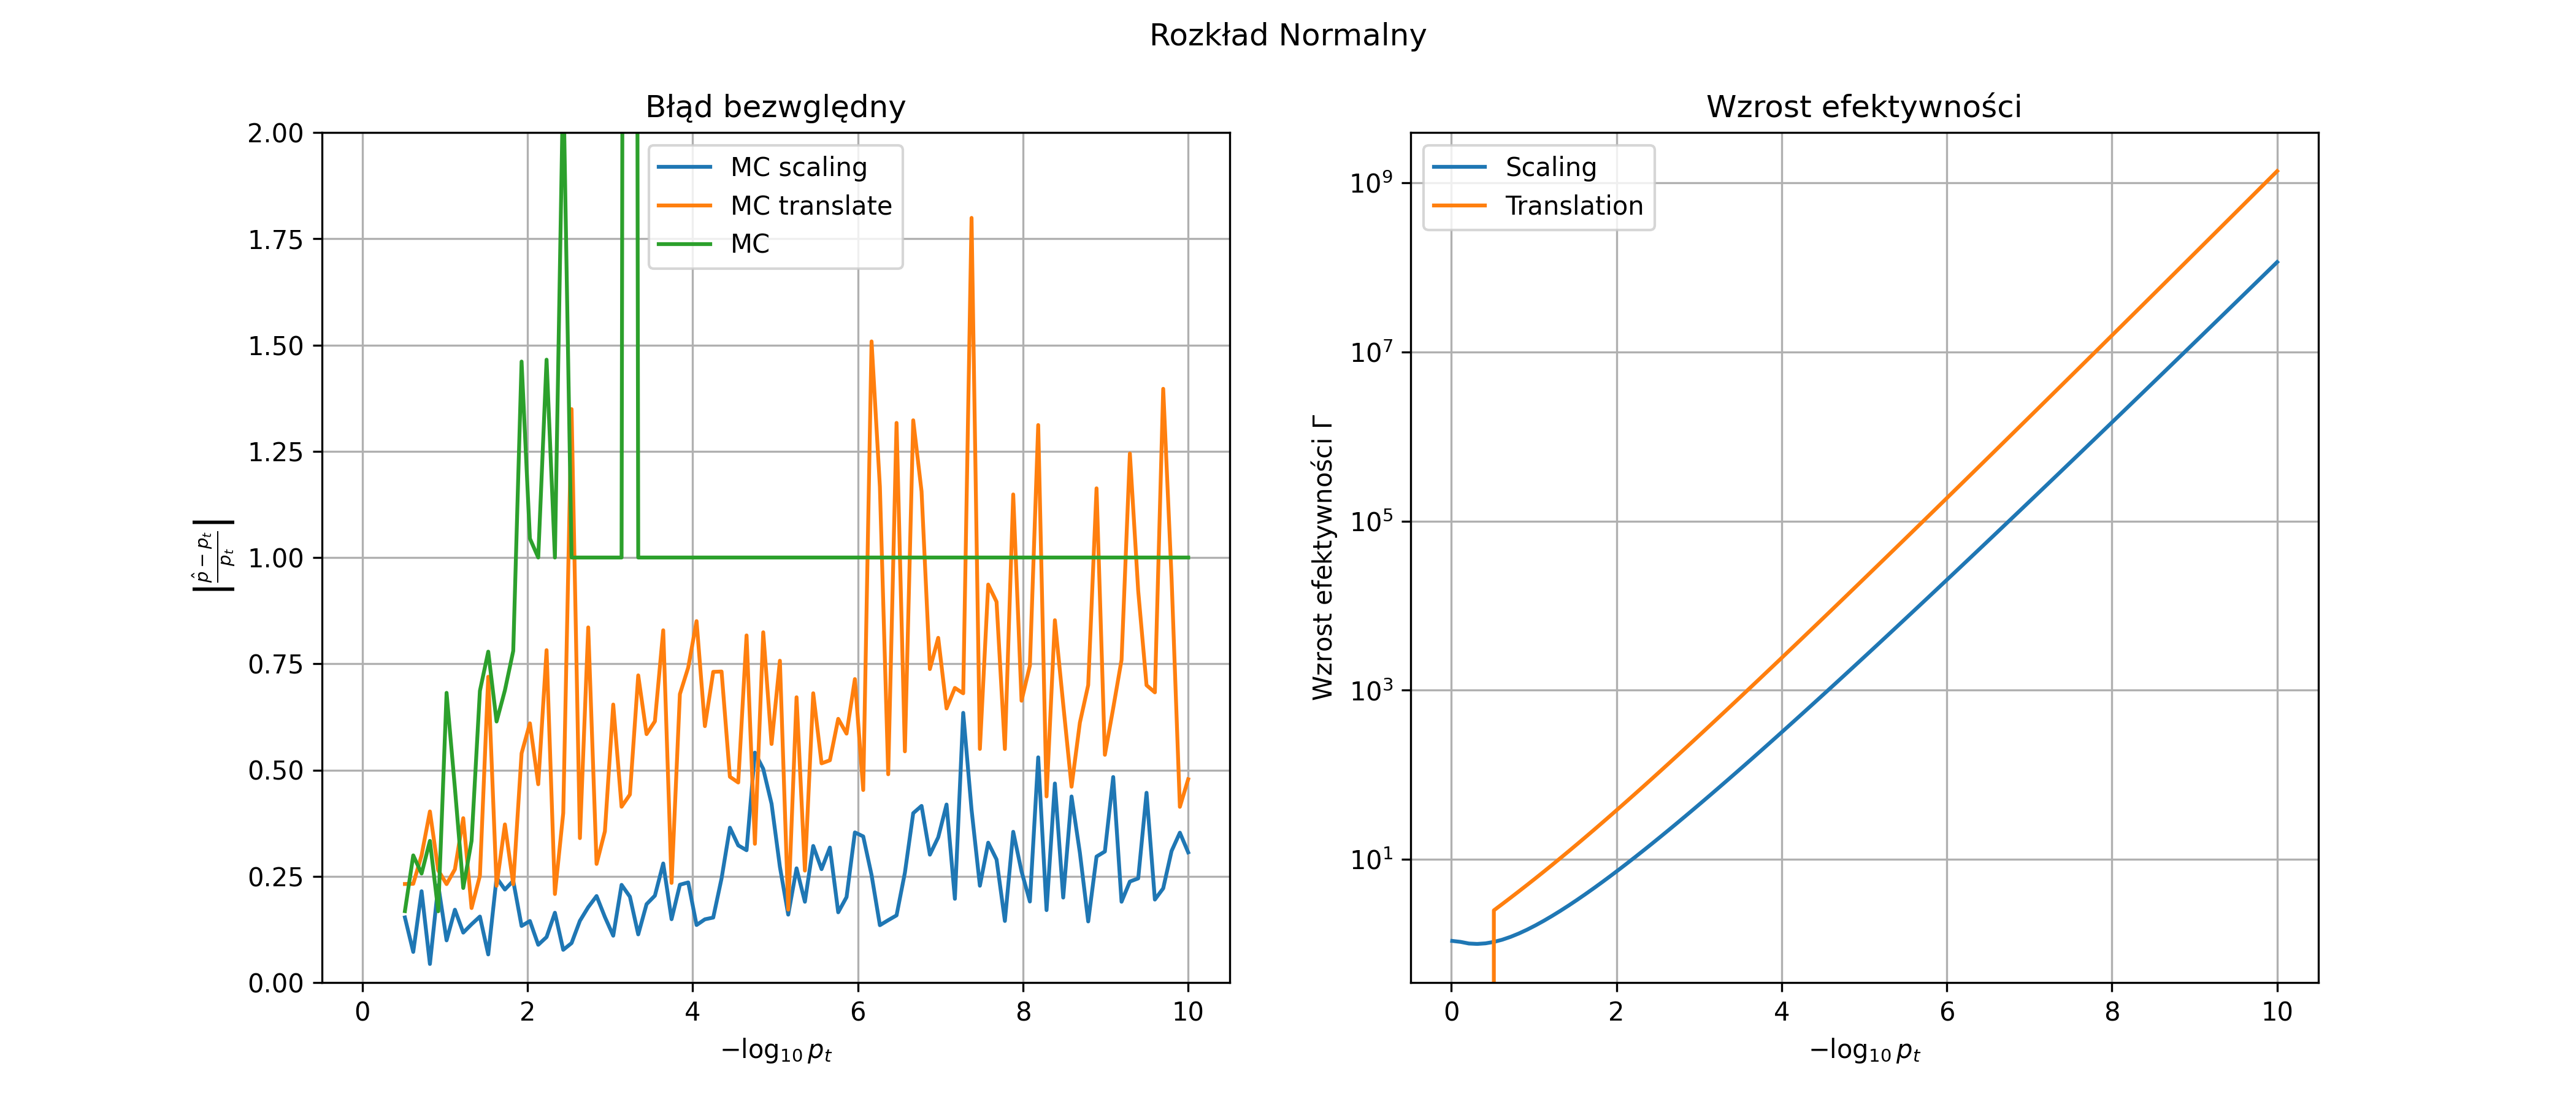
\includegraphics[width=\textwidth, height=\textheight, keepaspectratio]{figures/current/subblots_normal.png} \end{figure} \end{frame}

\begin{frame}{Numerical testing}{Weibull distribution}\begin{figure} 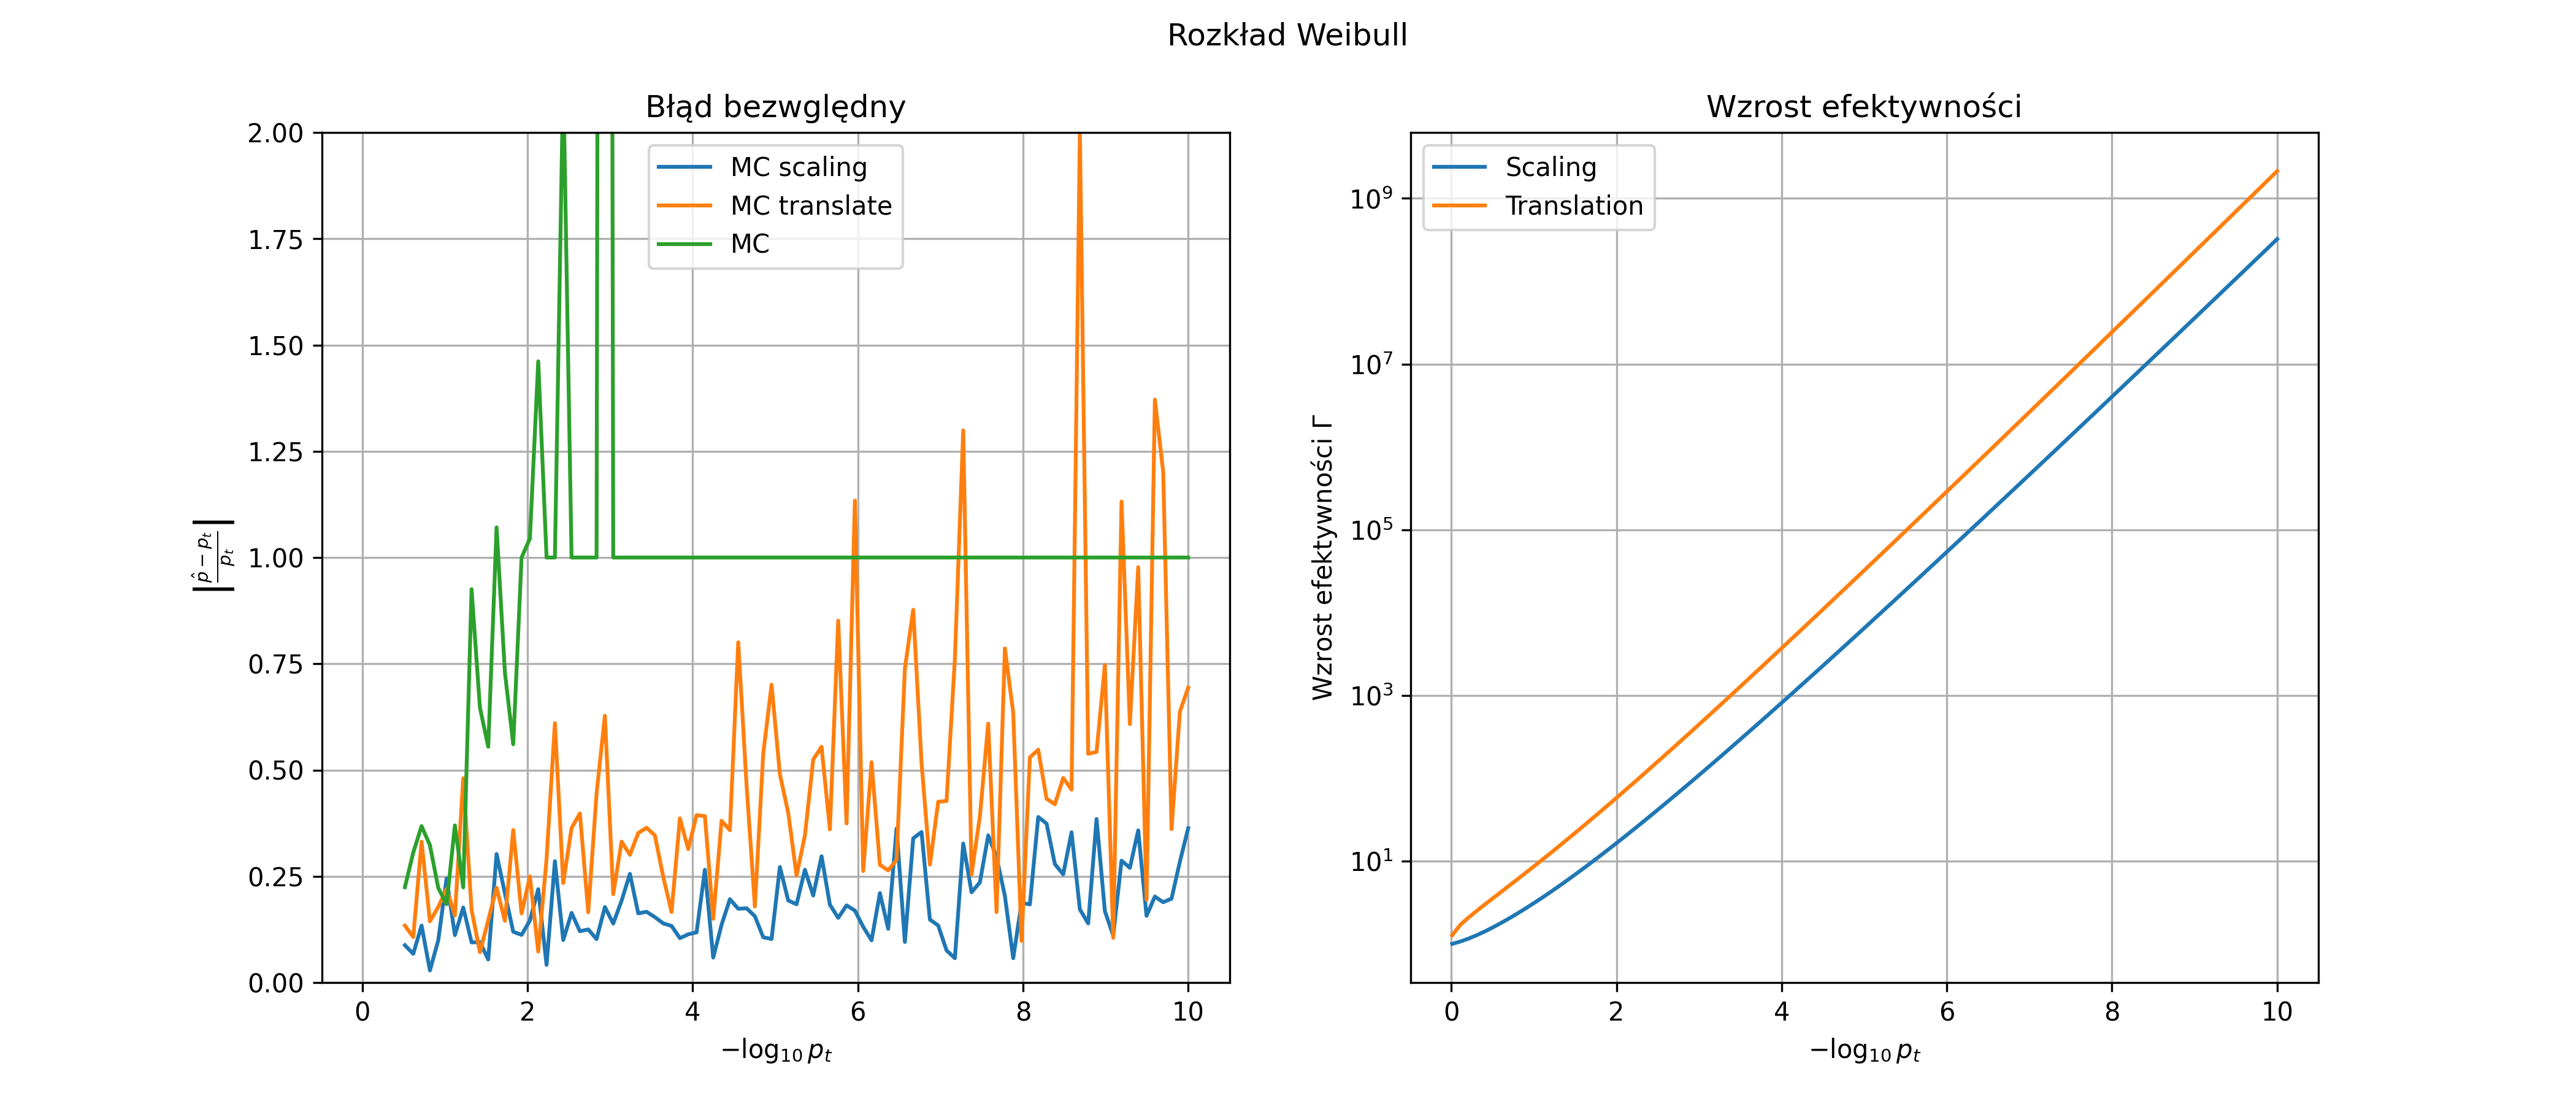
\includegraphics[width=\textwidth, height=\textheight, keepaspectratio]{figures/current/subblots_weibull.png} \end{figure} \end{frame}
eeeew

\begin{frame}{References}
 \bibliographystyle{apalike}
\nocite{*}
\bibliography{references} \end{frame}

\end{document}
